\chapter{Conclusiones}\label{cap5}

A lo largo de este trabajo se ha mostrado el proceso de desarrollo del Sistema AutoSA, en este capítulo se dará cierre al desarrollo mostrando como la implementación del el sistema AutoSA, dada en el Capítulo \ref{cap4}, satisface los requerimientos funcionales y no funcionales del Capítulo \ref{cap2} sentando así las bases para mostrar el cumplimiento de los objetivos del proyecto AutoSA expresados en el Capítulo \ref{cap1} enunciando los resultados obtenidos. Posteriormente se plantearán mejoras y extensiones al sistema.  

\section{Cumplimiento de requerimientos}
El en la sección \ref{sec:req-ana} se expusieron los requerimientos para el sistema AutoSA, estos requerimientos se presentan en dos grupos, funcionales y no funcionales. A continuación se mostrará evidencia del cumplimiento de tales requerimientos.

\subsection{Cumplimiento de requerimientos funcionales}
En la sección \ref{sec:req-fun} se enlistan los requerimientos funcionales que a continuación serán verificados:

\subsubsection{Automatización de los procesos en el Sistema de Abastecimiento}
Estos requerimientos (ver secciones \ref{sec:req-contestar} y \ref{sec:req-verificar}) automatizan los procesos descritos en la sección \ref{sec:desc-general} y son reflejados en los casos de uso CU-CONTESTAAR y CU-VERIFICAR (ver secciones \ref{cu-contestar} y \ref{cu-verificar} respectivamente), la implementación es mostrada en la sección \ref{sec:agente}. El usuario puede ejecutar las automatizaciones desde la herramienta Sahi de la siguiente forma:
\begin{itemize}
	\item Iniciar Sahi sobre el explorar de Internet (ver punto 1 de la Figura \ref{fig:ss-sahi})
	\begin{figure}[h]
		\centering
		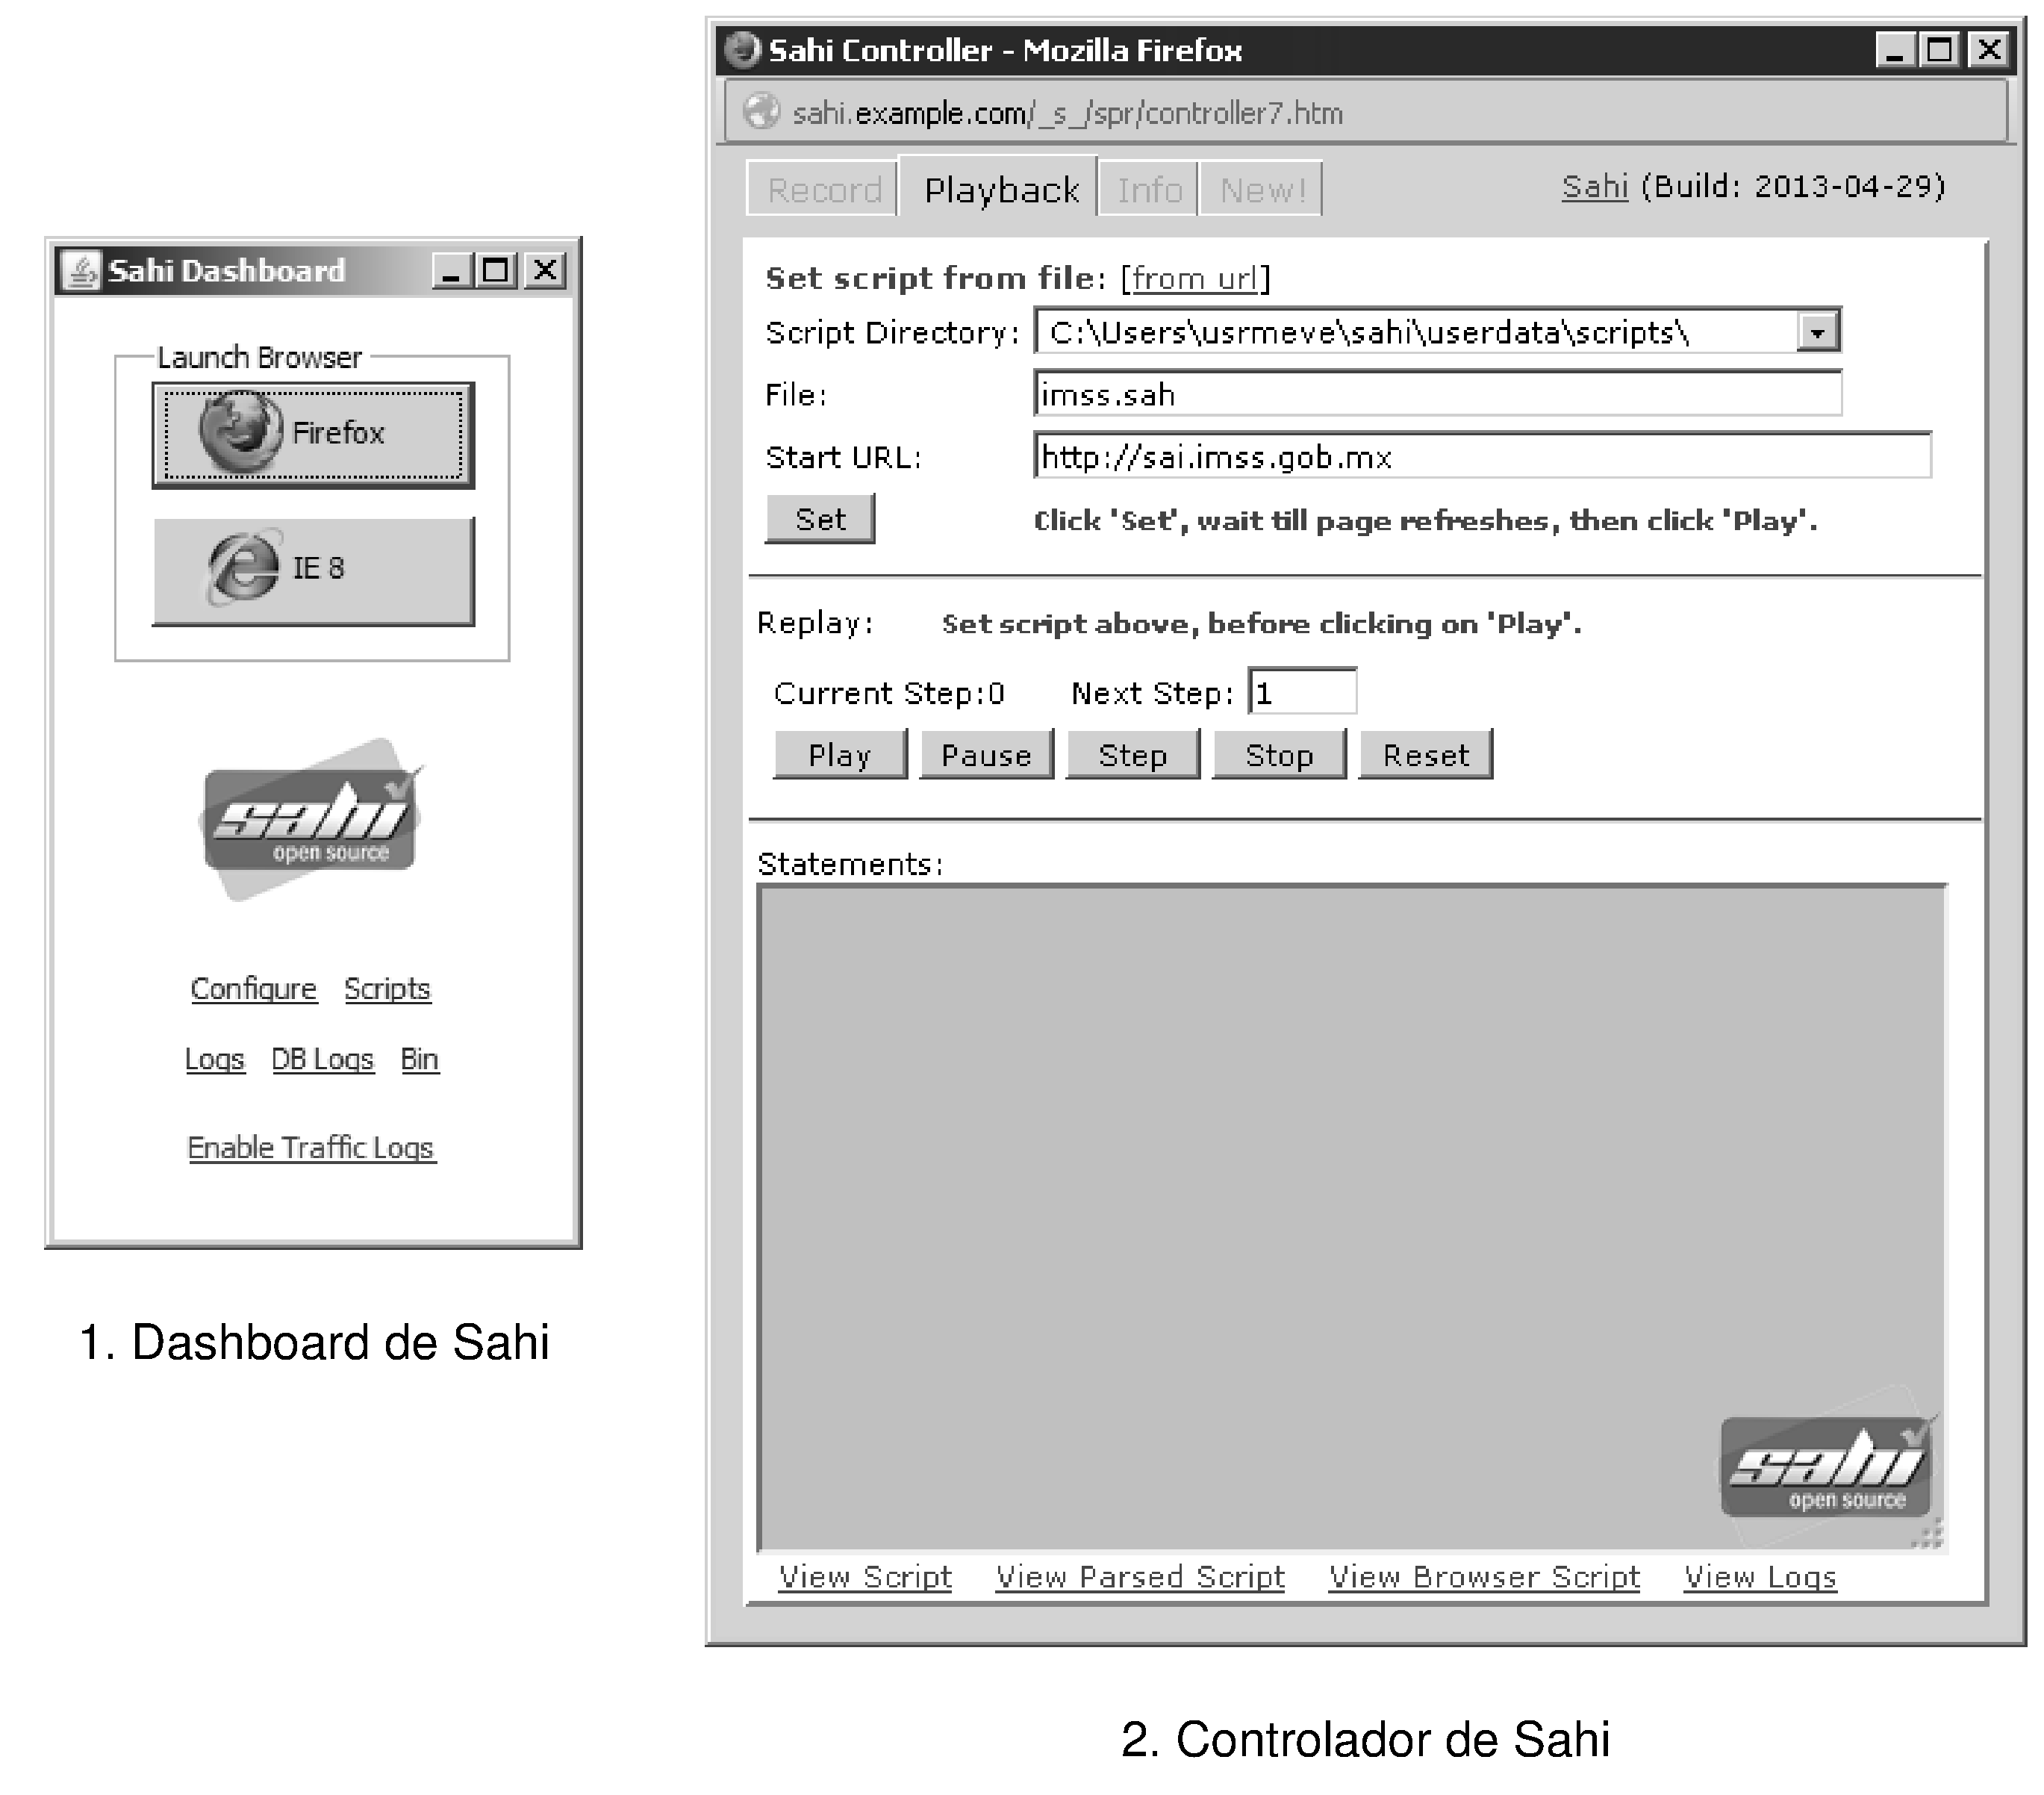
\includegraphics[scale=0.2]{ss-sahi}
		\caption{Interfaz de usuario de Sahi.}
		\label{fig:ss-sahi}
	\end{figure}

	\item Iniciar el controlador de Sahi y hacer los siguientes pasos (ver punto 2 de la Figura \ref{fig:ss-sahi}):
	\begin{enumerate}
		\item Seleccionar la rutina automatizada (contestar órdenes de reposición o verificación de órdenes de reposición)
		\item Ingresar la URL del Sistema de Abastecimiento
		\item Iniciar la ejecución.
	\end{enumerate}
\end{itemize}

\subsubsection{Interfaz WEB para la administración de órdenes de reposición contestadas}
La interfaz Web descrita en este requerimiento (ver sección \ref{sec:req-web-ui}) fue elaborada a lo largo de la sección \ref{sec:web-portal}, en particular los servicios de acceso y autorización fueron mostrados en el apartado 1 de la sección \ref{sec:backend}, así mismo, la pantalla de acceso fue descrita en el apartado 1 de la sección \ref{sec:frontend}.\\
Cabe mencionar que la pantalla de acceso es la primera pantalla que muestra la interfaz Web (ver Figura \ref{fig:ss-login}).
\begin{figure}[h]
	\centering
	\includegraphics[scale=1.8]{ss-login}
	\caption{Captura de pantalla de acceso a la interfaz Web.}
	\label{fig:ss-login}
\end{figure}

\subsubsection{Búsqueda de órdenes de reposición}
La pantalla para la búsqueda de órdenes de reposición es como se muestra al usuario la implementación del requerimiento de la sección \ref{sec:req-search}, la implementación de la pantalla y el comportamiento de esta es mostrado en el apartado 4 de la sección \ref{sec:frontend}. Por otra parte, la implementación de los servicios Web que consume la pantalla de búsqueda de órdenes de reposición son mostrados en el apartado 2 de la sección \ref{sec:backend}.\\
El la Figura \ref{fig:ss-search} se muestra la captura de pantalla de búsqueda de órdenes de reposición de la interfaz Web como se muestra al usuario.
\begin{figure}[h]
	\centering
	\includegraphics[scale=0.4]{ss-search}
	\caption{Captura de pantalla de búsqueda de órdenes de reposición.}
	\label{fig:ss-search}
\end{figure}

\subsubsection{Visualización y edición de una orden de reposición}
Los requerimientos para visualización y edición de una orden de reposición, requerimientos \ref{sec:req-show} y \ref{sec:req-update} respectivamente, son plasmados en los casos de uso CU-VISUALIZAR y CU-EDITAR (secciones \ref{cu-visualizar} y \ref{cu-editar} respectivamente). En la implementación y en la interfaz de usuario se utiliza la misma pantalla, como se muestra en la Figura \ref{fig:ss-edit}, esta vista es descrita en el apartado 5 de la sección \ref{sec:frontend}. La implementación de los servicios Web que consume la pantalla son mostrados en el apartado 2 de la sección \ref{sec:backend}.
\begin{figure}[h]
	\centering
	\includegraphics[scale=0.4]{ss-edit}
	\caption{Captura de pantalla de búsqueda de órdenes de reposición.}
	\label{fig:ss-edit}
\end{figure}

\subsubsection{Generación de reportes}
La generación de reportes cumple con los requerimientos de las secciones \ref{sec:req-rep-contestadas}, \ref{sec:req-rep-layout} y \ref{sec:req-rep-canceladas}; mismos que son englobados en el caso de uso CU-GENERAR-REPORTE (ver sección \ref{cu-generar-reporte}). La implementación de la generación de reportes está descrita en la sección \ref{sec:gen-repport} así como los servicios Web que exponen esta funcionalidad son mostrados en el apartado 2 de la sección \ref{sec:backend}. La vista que se muestra al usuario es descrita en el apartado 2 de la sección \ref{sec:frontend}, en la Figura \ref{fig:ss-report} se observa la captura de pantalla como se muestra al usuario\footnote{Por acuerdo de confidencialidad no se puede mostrar el contenido de los reportes generados.}. 
	\begin{figure}[h]
		\centering
		\includegraphics[scale=0.5]{ss-report}
		\caption{Captura de pantalla de generación de reportes.}
		\label{fig:ss-report}
	\end{figure}

\subsubsection{Actualización de catálogos y estatus de órdenes de reposición canceladas}
Los requerimientos \ref{sec:req-catalogos} y \ref{sec:req-canceladas} son atendidos por el caso de eso CU-ACTUALIZAR-CATALOGO (ver sección \ref{cu-actualizar-catalogo}), la implementación de la actualización a los datos es dada en la sección \ref{sec:persistence-web}, y la implementación del servicio Web es mostrada en el apartado 2 de la sección \ref{sec:backend}. La implementación de la vista es mostrada en el apartado 3 de la sección \ref{sec:frontend}, en la Figura \ref{fig:ss-catalog} se observa la captura de pantalla de la vista como se muestra al usuario\footnote{Por acuerdo de confidencialidad no se puede mostrar el contenido de los catálogos.}.
\begin{figure}[h]
	\centering
	\includegraphics[scale=0.4]{ss-catalog}
	\caption{Captura de pantalla de administración de catálogos.}
	\label{fig:ss-catalog}
\end{figure}

\subsubsection{Navegación dentro de la interfaz web}
La implementación del requerimiento \ref{sec:req-nav-bar} es mostrada en la sección \ref{sec:frontend}, en la Figura \ref{fig:ss-nav-bar} se observa la captura de pantalla de la barra de navegación.
\begin{figure}[h]
	\centering
	\includegraphics[scale=0.4]{ss-nav-bar}
	\caption{Captura de pantalla de la barra de navegación.}
	\label{fig:ss-nav-bar}
\end{figure}


\subsection{Cumplimiento de requerimientos no funcionales}
En la sección \ref{sec:nonfunctional-req} se enlistan los requerimientos no funcionales que a continuación serán verificados.

\subsubsection{Sistema operativo capaz de ejecutar la máquina virtual de Java}
El sistema operativo fue provisto por la farmacéutica, quien aseguró la correcta ejecución de la máquina virtual de Java.

\subsubsection{Base de datos relacional SQL}
Al igual que el sistema operativo, la base de datos fue proporcionada por la farmacéutica.

\subsubsection{Uso de la herramienta Sahi para automatizar interacción con Sistema de Abastecimiento}
En el cumplimiento de los requerimientos funcionales 1 y 2 de la sección anterior y en la sección \ref{sec:agente} se muestra la implementación del módulo \textbf{Agente} utilizando Sahi.

\subsubsection{Las contraseñas de los usuarios para el acceso a la interfaz web deben ser almacenadas utilizando un algoritmo de cifrado}
En la sección \ref{sec:backend} se muestra la verificación y cifrado de la contraseña de un usuario\footnote{\textcolor{red}{Esto falta, se debe mostrar el cifrado utilizando algún estándar de salt o algún algoritmo de cifrado}}.


\section{Resultados}

\subsection{Cumplimiento de objetivos principales}
El objetivo principal del proyecto AutoSA, definido en la sección \ref{sec:objetivo-principal}, es lograr reducir el tiempo que le toma a la farmacéutica contestar las órdenes de reposición en el Sistema de Abastecimiento y detectar con mayor rapidez las órdenes que han sido canceladas por el Instituto de Salud.\\
Gracias a la liberación del sistema AutoSA se logró reducir el tiempo de atención de 24 horas hombre al día a 2 horas hombre al día. Mientra que la detección de órdenes de reposición canceladas antes del sistema AutoSA se efectuaba cada tercer día, ahora con el sistema AutoSA se efectúa a diario por lo que la ventana de tiempo para impedir el envío de medicamentos no solicitados ha aumentado tres veces.

\subsection{Cumplimiento de objetivos secundarios}

\begin{enumerate}
	\item Reducción del error humano en relación a la manipulación de la información.
	\item Ahorro de recursos en la entrega de medicamentos no solicitados.
	\item Reducción de tiempo en cuanto a la respuesta de órdenes de reposición.
	\item Consistencia en los datos respecto a la generación de reportes estadísticos sobre las órdenes de reposición procesadas.
\end{enumerate}
Por lo anterior los afiliados del Instituto se verán beneficiados, pues los medicamentos estarán disponibles con mayor frecuencia en las clínicas y hospitales.

\section{Trabajo futuro}
\begin{itemize}
	\item 
\end{itemize}

\section{Conclusiones finales}

Durante este proyecto y toda mi carrera profesional he aplicado los conocimientos que adquirí en la Facultad de Ciencias sobre programación y paradigmas de programación, lógica, bases de datos, redes de computadoras, ingeniería de software, análisis y diseño de algoritmos, teoría de códigos, álgebra lineal. También adquirí habilidades y costumbres como buscar y aprender por mi mismo nuevas tecnologías, esto me ha apoyado para mantenerme en constante actualización haciendo que hasta la fecha sea un buen elemento en mis equipos de trabajo\footnote{\textcolor{red}{¿Muy cursi?}}.
